\documentclass[serif,9pt]{beamer}
\usepackage{color,listings}
\usepackage{ragged2e}
\usepackage[spanish]{babel}
\usepackage[utf8]{inputenc}
\usepackage{graphicx}

\definecolor{dkgreen}{rgb}{0,0.6,0}
\definecolor{gray}{rgb}{0.5,0.5,0.5}
\definecolor{mauve}{rgb}{0.58,0,0.82}
\definecolor{lgray}{rgb}{0.99,0.97,0.95}
\newcommand{\X}{\textbf{X}}
\newcommand{\Y}{\textbf{Y}}
\newcommand{\Z}{\textbf{Z}}
\newcommand{\G}{\textbf{G}}
\newcommand{\R}{\textbf{R}}
\newcommand{\V}{\textbf{V}}
\newcommand{\Q}{\textbf{Q}}
\newcommand{\h}{\textbf{H}}
\newcommand{\T}{\textbf{T}}

\def\E{\mathbb{E}}
\def\C{\mathbb{C}}
\def\N{\mathbb{N}}

\setbeamercovered{transparent}


\usetheme{Frankfurt}
%\usecolortheme{rose}
%\usecolortheme{lily}
\usepackage{amsmath, multirow}
%\usepackage{color, amsmath, wrapfig, anysize, graphicx, hyperref, amsthm, fancyhdr, amssymb,geometry,amsfonts,float}

\newcommand{\ds}{\displaystyle}


\titlegraphic{
\includegraphics[width=4cm]{utfsm.eps}}%
   %\includegraphics[width=4cm]{fig/inria.eps}}

\begin{document}
\title{Current Investigation\\ Toward a Security Reference Architecture of Web Browser} 
\author[Paulina Silva Ghio]{\textsc{Paulina Silva Ghio} \\ \medskip
\small{}
\medskip
\url{pasilva@alumnos.inf.utfsm.cl}}
\institute[]{}
\date{22-03-2016/23-03-2016.}

\begin{frame}[plain]
\titlepage
\end{frame}


\begin{frame}
\frametitle{Index}
\tableofcontents
\end{frame} 


\section{Introduction}
\subsection{Context}
\begin{frame}
	\frametitle{Context}

	\begin{itemize}
		\item<1-> Web Browser's war in the nineties. 
		\item<1-> Built and fix.
		\item<1-> Web Browser: a tool used daily.
		\item<2-> Common user uses its services.
		\item<2-> Many type of implementations.
		\item<2-> Web 2.0 y 3.0: AJAX (Asynchronous Javascript and XML).
	\end{itemize}
	\begin{figure}[h]
	    \centering
	    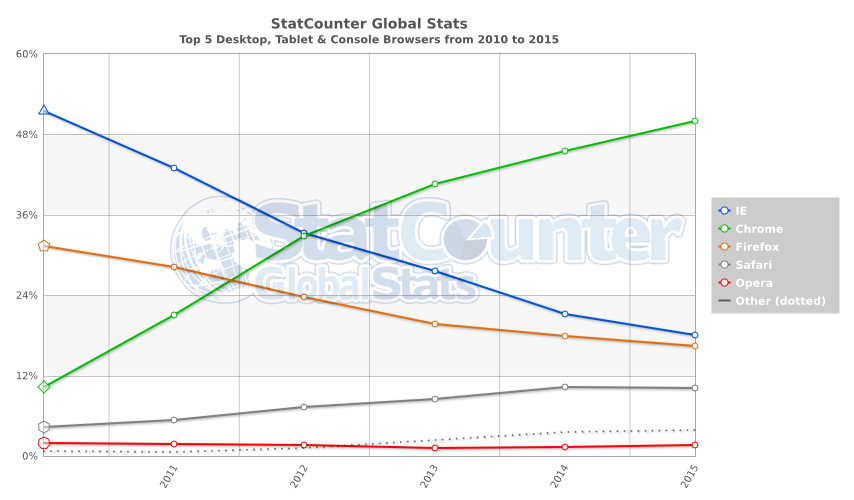
\includegraphics[scale=0.3]{figures/StatCounter-browser-ww-yearly-2010-2015.png}
	    \caption{Market Percentaje of each Browser. Cite: \cite{statBrow}}
	    \label{fig:UsageShare}
	\end{figure}
\end{frame}

% \subsection{Actualidad}
% \begin{frame}
% 	\frametitle{Actualidad}
% 	\begin{itemize}
% 		\item Sistemas actuales son muy complejos.
% 		\item Es necesario utilizar metodologías que aseguren: Requerimientos Funcionales y No-Funcionales.
% 		\item Defectos y errores en el Software generan vulnerabilidades.
% 		\item La Seguridad es un costo ``extra", a veces no considerado.
% 	\end{itemize}
% 	\begin{block}{Las vulnerabilidades...}
% 		Ocurren por que no se ha tomado en cuenta la seguridad en el desarrollo.
% 	\end{block}
% \end{frame}

\subsection{Motivation}
\begin{frame}
	\frametitle{Motivation}
	\onslide{Browser is an indispensable tool, this lets:}
	\begin{itemize}
		\item<1-> New ways of interacting.
		\item<1-> Lower building costs for a client program.
		\item<2-> Already implemented a lot of robust security features in the browser.
		\item<2-> Reuse.
	\end{itemize}
	
	\begin{block}{Principal Concerns}
	\begin{itemize}
		\item<3-> Systems which are called by users using a browser.
		\item<4> Stakeholders involved: browser's user, host's user and the external service used.
	\end{itemize}
	\end{block}
\end{frame}

\section{Problem}
\subsection{Threats and Vulnerabilities}
\begin{frame}
	\frametitle{Threats and Vulnerabilities}
	\begin{columns}
	\column{0.5\textwidth}
	\begin{minipage}[c][0.4\textheight][c]{\linewidth}
	  \centering
	  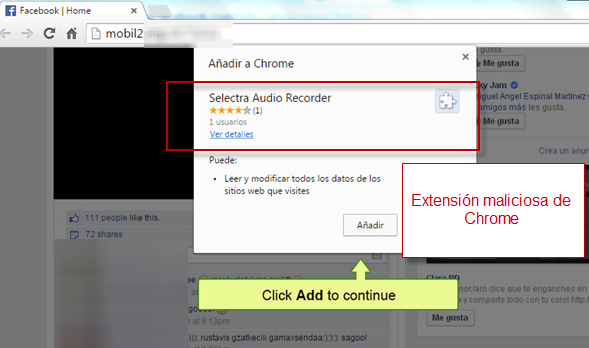
\includegraphics[scale=0.3]{figures/fbporn3.png}
	  \label{fig:Malware}
	\end{minipage}
	\begin{minipage}[c][0.4\textheight][c]{\linewidth}
	  \centering
	  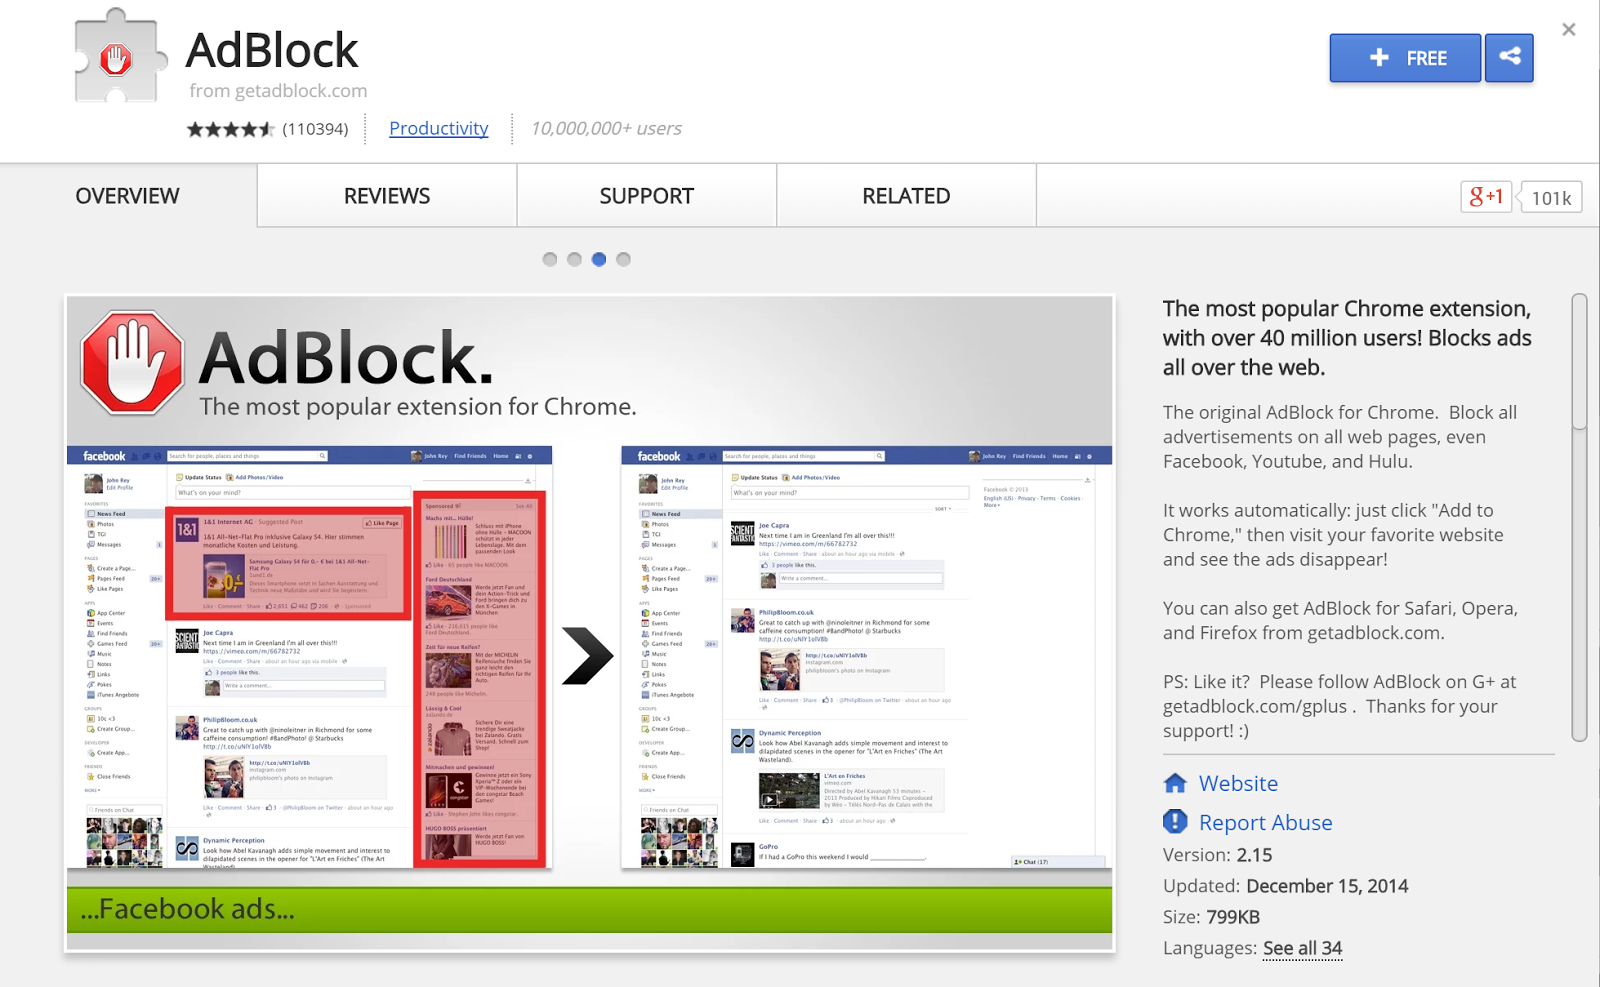
\includegraphics[scale=0.10]{figures/Adblock.png}
	  \label{fig:vulnExt}
	\end{minipage}
	\column{0.5\textwidth}
	\begin{minipage}[c][0.4\textheight][c]{\linewidth}
	  \begin{enumerate}
	  \item Installation of Malware and malicious Extensions.
	  \item Benign-but-buggy Extensions.
	  \item Man in the Browser.
	  \item Code Injection.
	  \end{enumerate}
	\end{minipage}
	\begin{minipage}[c][0.4\textheight][c]{\linewidth}
	  \centering
	  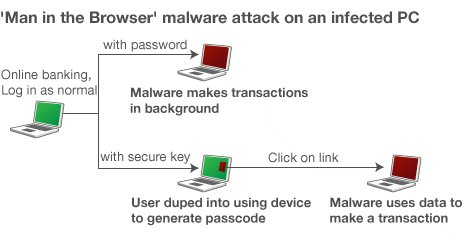
\includegraphics[scale=0.45]{figures/_58291188_malware_464v2.jpg}
	\end{minipage}
	\end{columns}
\end{frame}

\subsection{Problems}
\begin{frame}
	\frametitle{Problems}
	\begin{itemize}
		\item Lack of knowledge in browser's security aspects, could affect directly the development of applications and stakeholders. 
		\item Scarce documentation and none unification of concepts. No formal descriptions for browser related concepts.
	\end{itemize}
\end{frame}

\section{Theoretical Framework}
\subsection{Reference Architecture (RA)}
\begin{frame}
	\frametitle{Reference Architecture (RA) for the browser}
		\begin{itemize}
			\item<1-> Specifies the decomposition of the systems into subsystems, interactions between these parts and functionality distribution between them.
			\item<1-> Captures the essence of the architecture through a collection of similar systems, using architectonic reuse.
			\item Currently, there is no consensus in how to define an RA, what should have and how should be built. We use architectural patterns.
			\item<2-> Describes concerns and quality attributes needed.
			\item<2-> Helps: developers, in general stakeholders.
			\item<3-> Compares design decisions.
			\item<3-> Holistic view of the system.
		\end{itemize}
\end{frame}

\subsection{Security Reference Architecture (SRA)}
\begin{frame}
	\frametitle{Security Reference Architecture (SRA)}
	\begin{itemize}
		\item<1-> Holistic view of security, taking into account the threats.
		\item<1-> Abstraction of defense mechanism described as security patterns.
		\item<2-> Unifies terminology.
		\item<2-> Can help to evaluate a system and its security requirements.
	\end{itemize}
\end{frame}


\subsection{Securing a RA}
\begin{frame}
	\frametitle{Securing a RA}
	\begin{itemize}
		\item<1-> We start from a list of use cases which describe the typical cloud uses and their associated roles. Lists of cloud use cases are shown in [Bad12], [nis11], and [Has13c]. 
		\item<2-> We analyze each use case looking for vulnerabilities and threats as in [Bra08]. This implies checking each activity in the activity diagram of the use cases to see how it can be attacked. This approach results in a systematic enumeration of threats.
		\item<3-> We use the list of threats from [Has13a] to confirm these threats and to find possible further vulnerabilities and threats.
		\item<4-> These threats are expressed in the form of misuse patterns. We developed some misuse patterns for Cloud Computing in [Has13b], we show more later.
		\item<5-> We apply policies to handle the threats and we identify security patterns to realize the policies.  There are also regulatory policies which are realized as security patterns.
		\item<6-> SRA can be used as a guideline to specify what the customer wants, and cmply to SLA of Cloud services

	\end{itemize}
\end{frame}


\subsection{RA and SRA}
\begin{frame}
	\frametitle{RA and SRA}
	\begin{columns}
		\column{0.5\textwidth}
		\begin{minipage}[c][0.4\textheight][c]{\linewidth}
		  \centering
		  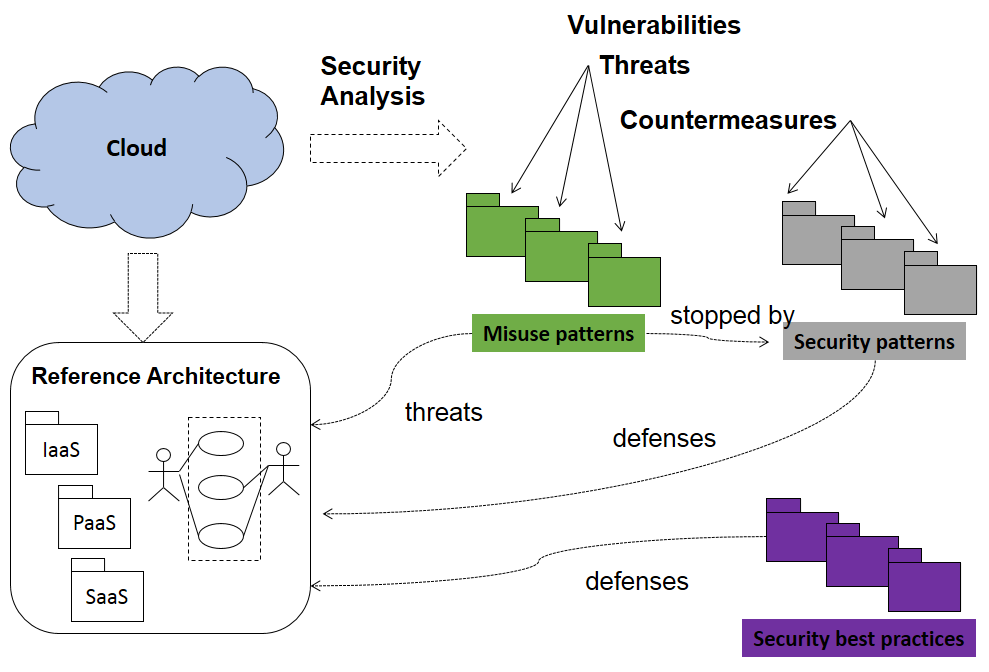
\includegraphics[scale=0.26]{figures/SRA.png}
		  \label{fig:Malware}
		\end{minipage}
		%\column{0.5\textwidth}
		\begin{minipage}[c][0.4\textheight][c]{\linewidth}
		  \centering
		  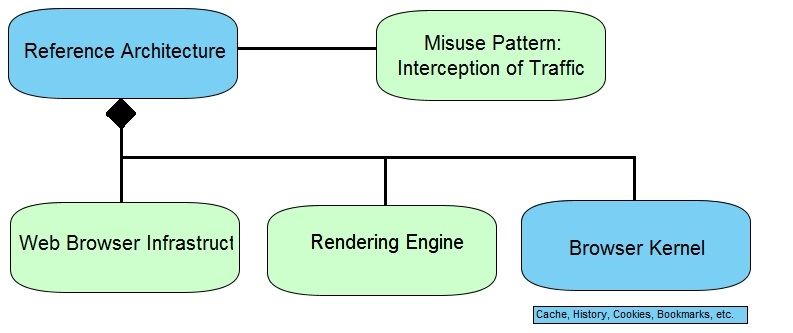
\includegraphics[scale=0.36]{figures/relations.jpg}
		  \label{fig:vulnExt}
		\end{minipage}
	\end{columns}
\end{frame}



\begin{frame}
	\frametitle{RA and SRA}
	\begin{itemize}
		\item<1-> RAs and SRAs are not implementable, they are abstract artifacts, their evaluation is based on completeness (they cover all concrete RAs as special cases), precision (UML modeling), understandability, extensibility (produced by the use of patterns).
		\item<1-> Value: 
			\begin{itemize}
				\item<2-> can be used to produce new concrete architectures
				\item<2-> can be used to analyze the effect of threats
				\item<3-> can be used to define monitoring points
				\item<3-> can be used as the basis of Service Contracts
				\item<3-> can be used to define use cases.
			\end{itemize}
		\item<4-> Browser: Until now, there is no clear and precise model of the actual requirements and components. Only old models.
	\end{itemize}
\end{frame}


\subsection{Misuse Patterns}
\begin{frame}
	\frametitle{Misuse Patterns}
	\begin{itemize}
		\item<1-> Describes from the point of view of the attacker, how an attack can be done (which units uses and how), analizes the ways of stopping the attack by enumerating the possible security patterns that could be used, and describes how to trace back the attack once it has occured (recolection of forensic data).
		\item<2-> Let teach and communicate possible ways how a system can be misused.
	\end{itemize}
\end{frame}


\subsection{State of Art}
\begin{frame}
	\frametitle{State of Art}
	\begin{itemize}
		\item Have not found updated works about Reference Architectures of the Browser. The work of Grosskurth et al. \cite{preprint-grosskurth-browser-archevol} is close, but the technique is different.
		\item Works: 
		\begin{itemize}
			\item<1-> Larrondo et al. \cite{535061}: analyzes the browser and obtains a Domain Model,  an Object Model, a Feature Tree which describes structure and functionality of the browser.
			\item<2-> Grosskurth et al. \cite{2005-grosskurth-browser-refarch,preprint-grosskurth-browser-archevol}: Reverse engineering tool to obtain a high-level architecture of open-source browsers: Mozilla y Konqueror.
			\item<3-> Godfrey et al. \cite{Godfrey2000}: similar to the above but only for Mozilla, and also obtained architectural views of the system.
			\item<4-> Lwin \cite{Lwin2009}: proposes a browser called Anfel SOFT, with AI to improve user's experience.
		\end{itemize}
		\item<5-> Scarse and poor documentation. None unification of concepts.
		\item<5-> As for a SRA, thre was no work found.
	\end{itemize}
\end{frame}


\section{Proposal}
\subsection{General and specific objectives/goals}
\begin{frame}
	\frametitle{General and specific objectives/goals}
	\begin{block}{General objective}
		\begin{small}
		\begin{itemize}
			\item<1-> Build an organized body of information about the Web Browser and its security.
			\item<1-> Systematize, organize and classify adquiered knowledge in a document, with a semi-formal format.
			\item<1-> Better comprehension of browser's security.
		\end{itemize}
		\end{small}
	\end{block}
	\begin{block}{Specific objectives}
		\begin{small}
			\begin{itemize}
				\item<2-> A guide to comunicate relevant concepts.
				\item<2-> Improve our Reference Architecture and continue our misuse pattern catalog. 
				\item<2-> Build a conceptual model of browser's security, a Security Reference Architecture.
				\item<3-> Get to know how social engineering can affect the browser.
				\item<3-> Use Experimental Software Engineering techniques.
			\end{itemize}
		\end{small}
	\end{block}
\end{frame}


\subsection{Hypotesis}
\begin{frame}
	\frametitle{Hypotesis}	
	\begin{block}{Main Hypotesis}
			H1: The definition of a Security Reference Architecture for the Web Browser allows to abstract and capture main structural aspects, its behavior and security related requirements.
	\end{block}
	% \begin{block}{Otra posible hipótesis}
	% 	%\begin{itemize}
	% 	H2: El uso de una Arquitectura de Referencia de Seguridad permite añadir seguridad al desarrollo de aplicaciones web.
	% 		%\item H3: El uso de una Arquitectura de Referencia de Seguridad permite la construcción de Browser Seguros.
	% 	%\end{itemize}
	% \end{block}
\end{frame}

\subsection{Validation}
\begin{frame}
	\frametitle{Validation}	
	\begin{itemize}
	\item<1-> Reference Architecture and Security Reference Architecture are not implemented. They are abstract models.
	\item<1-> Experts opinions.
	\item<2-> *PLoP conferences and ``shepherding" process. Conferences: AsianPLoP y EuroPLoP.
	\item<2-> Experimental Software Engineering to validate or reject hypotesis. 
	\end{itemize}
\end{frame}

\subsection{Work already done}
\begin{frame}
	\frametitle{Work already done}
	\begin{itemize}
		\item RA and misuse patterns.
			\begin{itemize}
				\item<1-> \textbf{Browser Infrastructure Pattern}. A pattern which abstracts web browser's architecture implementations and request/response communication (mostly, since implementations may differ).
				\item<1-> \textbf{Web Content Renderer Pattern}. A pattern which abstracts th interior of the web browser's Renderer Engine.
				\item<2-> \textbf{Browser Kernel Pattern} (not ready yet). A pattern which abstracts the principal component of the browser, like cache, cookies, bookmarks, network communication, etc.
				\item<3-> \textbf{Misuse Pattern: Interception of Traffic}. A pattern which abstract a misuse that could occur in the web browser when an attacker beforehand achieves a social engineering attack. When the SE attack is succesful, the misuse is capable of intercepting the messages between Browser Kernel and Web Content Renderer.
			\end{itemize}
		\item<4-> AsianPLoP and EuroPLoP.
	\end{itemize}
\end{frame}

\section{Side work}
\begin{frame}
	\frametitle{Side work}
	\begin{itemize}
		\item<1-> Fondecyt Project: Software Development Initiatives to Identify and Mitigate Security Threats -- A Systematic Mapping.
			\begin{itemize}
				\item<2-> A systematic mapping has been conducted to cover the existent technologies for identification and mitigation of security threats.
				\item<2-> A total of 10 different techniques covering threats identification and 8 covering the mitigation of threats were found. 
				\item<3-> All the initiatives were integrated to at least one activity of the Software Development Lifecycle (SDLC), while 7 show signs of being adopted in the industry. 
				\item<3-> The mapping found only 15 studies that covered 11 different iniatiatives. 
				\item<4-> Only two techniques presented scientific evidence of its results through controlled experiments, while others selected studies presented informal case studies or examples.
			\end{itemize}
		\item<5-> Fondecyt Project: Research
			\begin{itemize}
				\item<6-> A Theoretical Framework for quality assessment of security metrics.
				\item<7-> How to evaluate security in software development
			\end{itemize}
	\end{itemize}
\end{frame}


\begin{frame}
	\frametitle{Questions?}
	¡Muchas Gracias!, Thank you!, Arigatou Gozaimashita!, Grazie!
\end{frame}

\bibliography{refTodas}
\bibliographystyle{IEEEtran}

\end{document}

